{\begin{abstract}
本章では,Polylibの主なAPIの利用方法を説明します.
\end{abstract}

% 
\graphicspath{{./fig_api/}}

%
\section{単一プロセス版の主なAPIの利用方法}

本節では単一プロセス版Polylibの主なAPI利用方法を,API呼び出し順に沿って説明します.

単一プロセス版PolylibのAPIを利用する手順は下図の通りです.

\begin{figure}[H]
 \centering
 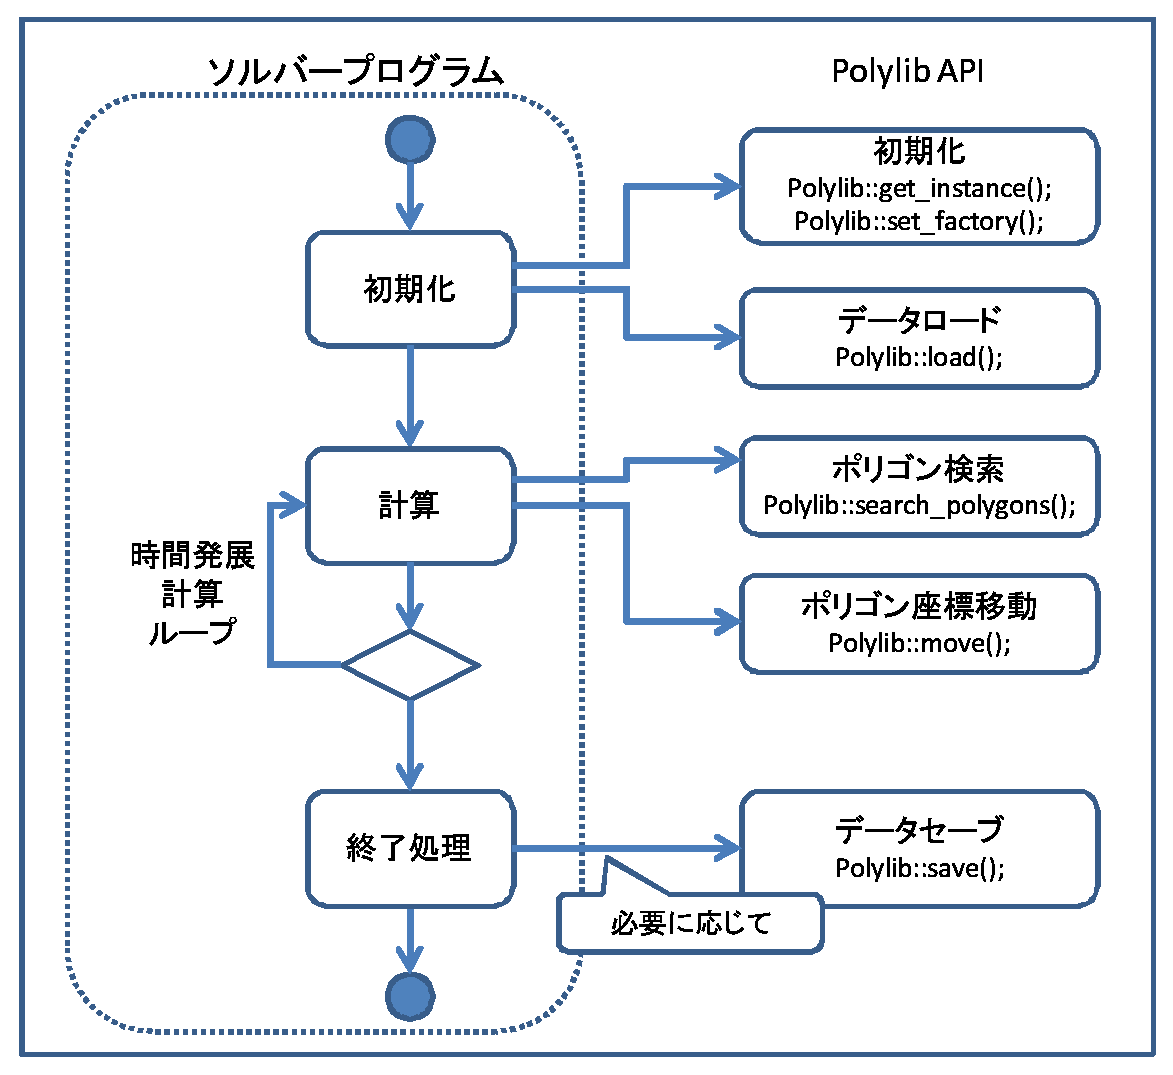
\includegraphics[width=12cm]{clip004.eps}\\
 \caption{API利用手順(単一プロセス版)}
\end{figure}

%
\subsection{初期化API}

%
\subsubsection{Polylibインスタンスの生成}
 \\

\begin{program}
	static Polylib* Polylib::get_instance();
\end{program}

Polylibはsingletonクラスのため,ユーザプログラム中からPolylibインスタンスを明示的に生成する
必要はありません.StaticメソッドであるPolylib::get\_instance()を呼び出すことで,プロセス内唯一
のPolylibインスタンスが返却されます.

また,Polylib::get\_instance()により返却されたインスタンスをユーザプログラムで明示的に消去する
必要はありません.インスタンスはプロセス終了時に自動的に消去されます.

%
\subsubsection{PolygonGroup派生クラスインスタンス生成ファクトリークラスの設定}
 \\

\begin{program}
	void Polylib::set_factory(
		PolygonGroupFactory *factory
	);
\end{program}

ユーザが定義するPolylgonGroup派生クラスを利用する場合,その派生クラスインスタンスの生成方法を
記述したPolygonGroupFactory派生クラスインスタンスを,本メソッドを利用してPolylibに登録する必要
があります.

PolylgonGroup派生クラスを利用しないのであれば,本APIを呼び出す必要はありません.

PolygonGroup派生クラスの具体的な利用法については後述のチュートリアルを参照してください.

%
\subsection{データロードAPI}

\begin{program}
	POLYLIB_STAT Polylib::load(
		std::string config_name = "polylib_config.xml"
	);
\end{program}

引数config\_nameで指定されたPolylib初期化ファイルを読み込み,そこに記述された内容に基づきポリゴン
グループ階層構造をオンメモリに生成します.そして最下層ポリゴングループに指定されたSTLファイルを
読み込み,三角形ポリゴン情報のインスタンスの生成と,ポリゴン検索用KD木の生成を行います.

引数config\_name が指定されなかった場合,デフォルト初期化ファイル名である"polylib\_config.xml"を
カレントディレクトリから読み込みます.

%
\subsection{検索API} \label{search_api}

\begin{program}
	std::vector<Triangle*>* Polylib::search_polygons(
		std::string	group_name,
		Vec3f		min_pos,
		Vec3f		max_pos,
		Bool		every
	)const;
\end{program}

ポリゴングループ名group\_nameで指定されたグループ階層構造下から,位置ベクトルmin\_posとmax\_posにより
指定される矩形領域に含まれる三角形ポリゴンを検索します.

引数group\_nameはポリゴングループ名称フルパスで指定します.ポリゴングループ名称フルパスとは,階層
最上位のポリゴングループ名称から,当該グループ名称までを'/'でつなげたものです.たとえば,階層最上位
のポリゴングループ名が"group\_A"でその直下にある"group\_B"内のポリゴンを検索する場合,引数group\_nameに
指定する文字列は以下の通りです.

\begin{program}
	"group_A/group_B"
\end{program}

引数everyの指定方法は以下の通りです.

\begin{itemize}
 \item ture:	3頂点が全て指定領域内に含まれる三角形を検索
 \item false:	一部でも指定領域と交差する三角形を検索
\end{itemize}

返却されたstd::vectorインスタンスは,呼び出し側で消去する必要がありますが,その要素であるTriangle型
ポインタの指し示すTriangleインスタンスを消去してはいけません.

%
\subsection{ポリゴン座標移動API}

\begin{program}
	POLYLIB_STAT Polylib::move(PolylibMoveParams& param);
\end{program}

Polylib管理下にあるmoveメソッド実装済のPolygonGroup派生クラスに所属する三角形ポリゴンの座標を,move
メソッドに実装された座標移動関数に基づきその頂点座標を変更します.

引数paramは,PolygonGroup派生クラスmoveメソッドの引数に渡されます.PolylibMoveParamsクラス定義は以下
の通りです.

\begin{program}
	class PolylibMoveParams {
	public:
		int m_current_step;	/*現在の計算ステップ番号*/
		int m_next_step;	/*移動後の計算ステップ番号*/
		double m_delta_t;	/*1計算ステップあたりの時間変異*/
	};
\end{program}

moveメソッドの実装方法の実際については,後述のチュートリアルを参照してください.

%
\subsection{データセーブAPI} \label{datasave_api}

\begin{program}
	POLYLIB_STAT Polylib::save(
		std::string	*p_fname,
		std::string	format,
		std::string	extend = ""
	);
\end{program}

本API呼び出し時点でのグループ階層構造をPolylib初期化ファイル形式に,三角形ポリゴン情報を
STLファイルに出力します.

引数p\_fnameは出力引数で,p\_fname の指し示すstd::stringインスタンスに保存されたPolylib初期
化ファイル名が設定されます.

引数formatは,保存するSTLファイルの形式を指定します."stl\_a"の場合,アスキー形式で保存
します."stl\_b"の場合,バイナリ形式で保存します.

引数extendは,保存するファイル名に任意の文字列を付加します.ファイル名の書式については,
\ref{output_file}を参照してください.


\pagebreak

%
\section{MPI版の主なAPIの利用方法}

本節ではMPI版Polylibの主なAPI利用方法を,API呼び出し順に沿って説明します.

MPI版PolylibのAPIを利用する手順は下図の通りです.

\begin{figure}[H]
 \centering
 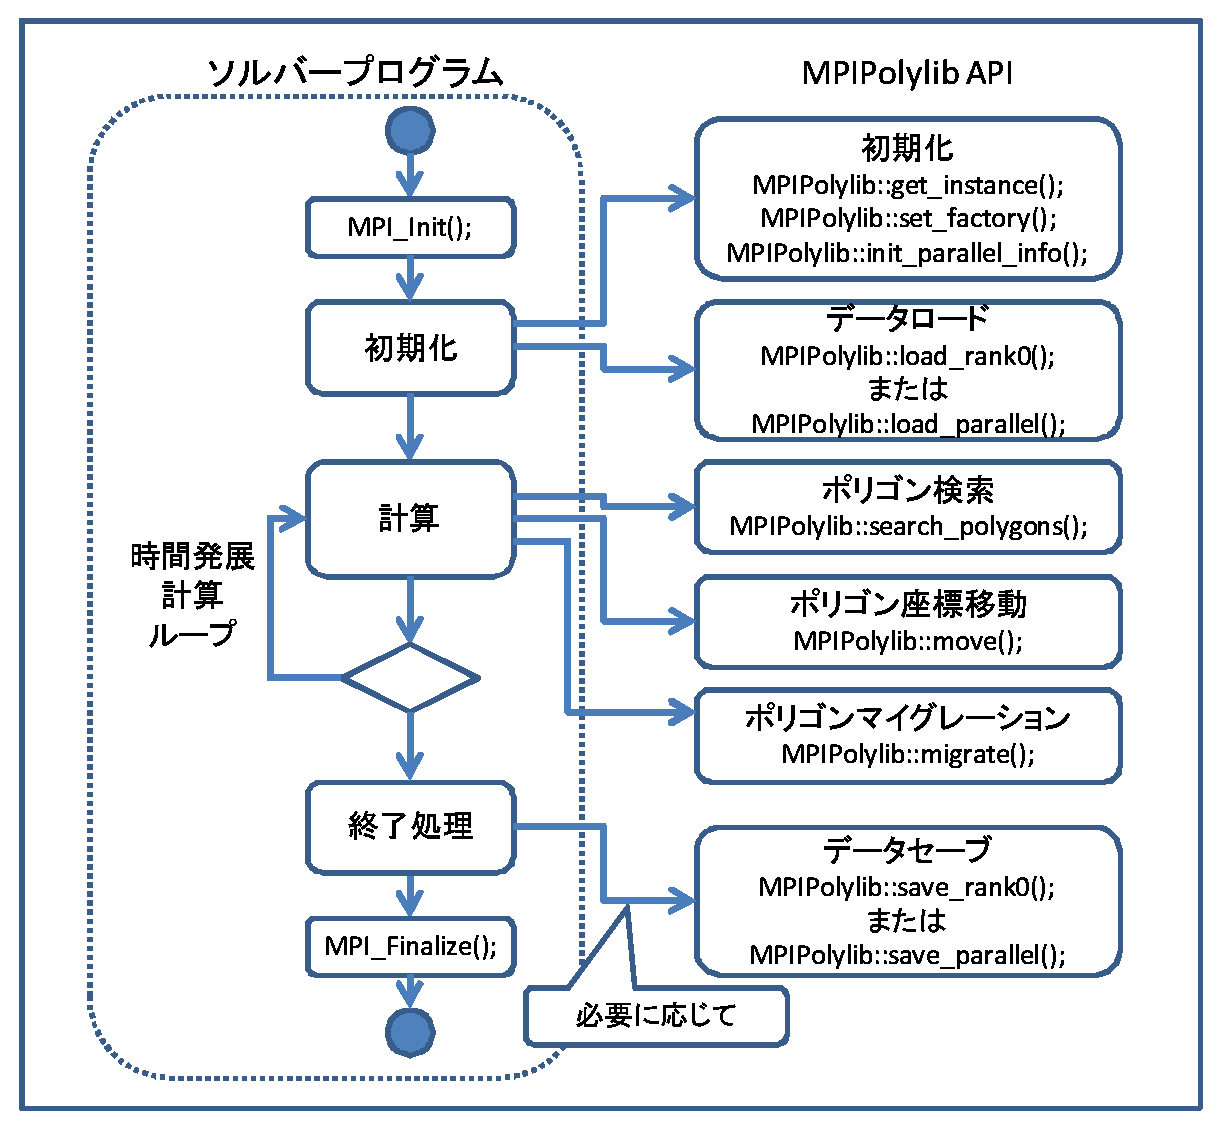
\includegraphics[width=12cm]{clip005.eps}
 \caption{API利用手順(MPI版)}
\end{figure}

%
\subsection{初期化API}

%
\subsubsection{MPIPolylibインスタンスの生成}
 \\

\begin{program}
	static MPIPolylib* MPIPolylib::get_instance();
\end{program}

MPIPolylibはPolylibクラスを継承し,MPI版機能を組み込んだクラスです.

Polylibクラス同様にsingletonクラスのため,ユーザプログラム中からMPIPolylibインスタンスを
明示的に生成する必要はありません.StaticメソッドであるMPIPolylib::get\_instance()を呼び出す
ことで,プロセス内唯一のMPIPolylibインスタンスが返却されます.

また,MPIPolylib::get\_instance()により返却されたインスタンスをユーザプログラムで明示的に
消去する必要はありません.インスタンスはプロセス終了時に自動的に消去されます.

%
\subsubsection{PolygonGroup派生クラスインスタンス生成ファクトリークラスの設定}
 \\

\begin{program}
	void MPIPolylib::set_factory(
		PolygonGroupFactory *factory
	);
\end{program}

ユーザが定義するPolylgonGroup派生クラスを利用する場合,その派生クラスインスタンスの生成方法
を記述したPolygonGroupFactory派生クラスインスタンスを,本メソッドを利用してPolylibに登録する
必要があります.

PolylgonGroup派生クラスを利用しないのであれば,本APIを呼び出す必要はありません.

PolygonGroup派生クラスの具体的な利用法については後述のチュートリアルを参照してください.

%
\subsubsection{並列計算情報の設定}
 \\

\begin{program}
	POLYLIB_STAT MPIPolylib::init_parallel_info(
		MPI_Comm     comm,
		float        bpos[3],
		unsigned int bbsize[3],
		unsigned int gcsize[3],
		float        dx[3]
	);
\end{program}

並列計算特有の値をMPIPolylibに設定します.各引数の意味は以下の通りです.

\begin{itemize}
 \item comm		MPIコミュニケータ
 \item bpos[3]	自ランクが受け持つ計算領域の基準座標
 \item bbsize[3]	自ランクが受け持つ計算領域のボクセル数
 \item gcsize[3]	自ランクが受け持つガイドセルのボクセル数
 \item dx[3]		ボクセル1辺の長さ
\end{itemize}

引数で設定された自ランク計算領域情報は,本API内部処理によりMPI通信により全ランクへ配信されます.

計算領域に関する各値の意味を下図に示します.

\begin{figure}[H]
 \centering
 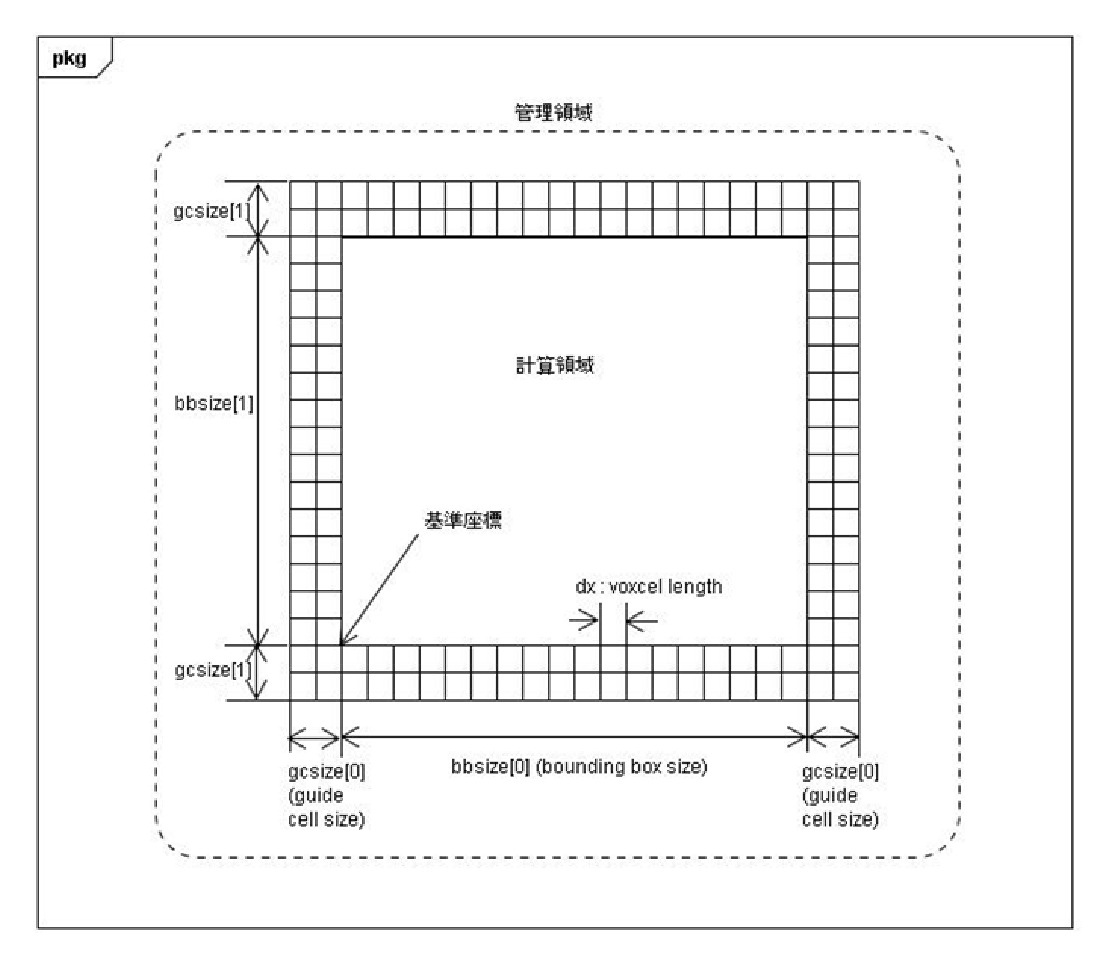
\includegraphics[scale=0.75]{clip006.eps}
 \caption{MPIPolylib::init\_parallel\_info() 各引数の意味}
\end{figure}


\subsection{データロードAPI}

\begin{program}
	POLYLIB_STAT MPIPolylib::load_rank0(
		std::string config_name = ""
	);

	POLYLIB_STAT MPIPolylib::load_parallel(
		std::string config_name = ""
		ID_FORMAT   id_format   = ID_BIN
	);
\end{program}

MPIPolylibでは2種類のデータロード系API があります.

MPIPolylib::load\_rank0は,rank0にてファイルを読み込み,他全ランクに対し,グループ階層情報と,
各ランクの担当領域ぶんのポリゴン情報をMPI通信にて配信します.

MPIPolylib::load\_paralellは,各ランクにてファイルを読み込みます.MPIPolylib::save\_parallelと
組み合わせて使用することで時間発展計算の中断/再開に対応しています.

いずれのAPIも,引数config\_nameで指定されたPolylib初期化ファイルを読み込み,そこに記述された
内容に基づきポリゴングループ階層構造をオンメモリに生成します.そして最下層ポリゴングループに
指定されたSTLファイルを読み込み,三角形ポリゴン情報のインスタンスの生成と,ポリゴン検索用KD木
の生成を行います.

引数config\_name が指定されなかった場合,デフォルト初期化ファイル名である"polylib\_config.xml"
をカレントディレクトリから読み込みます.

MPIPolylib::load\_paralellの引数id\_formatは,ロードする三角形IDファイルの形式を指定します.
未指定の場合,バイナリ形式の三角形IDファイルが存在するものとしてロード処理を行います.

%
\subsection{検索API}

\begin{program}
	std::vector<Triangle*>* Polylib::search_polygons(
		std::string	group_name,
		Vec3f		min_pos,
		Vec3f		max_pos,
		Bool		every
	)const;
\end{program}

MPIPolylibにおいても,検索APIは基底クラスPolylibのメソッドPolylib::search\_polygonsを利用します.

引数の説明は\ref{search_api}を参照してください.

\subsubsection{データセーブAPI}

\begin{program}
	POLYLIB_STAT MPIPolylib::save_rank0(
		std::string	*p_fname,
		std::string	format,
		std::string	extend = ""
	);

	POLYLIB_STAT MPIPolylib::save_parallel(
		std::string	*p_fname,
		std::string	format,
		std::string	extend = "",
		ID_FORMAT   id_format = ID_BIN
	);
\end{program}

MPIPolylibには2種類のデータセーブ系APIがあります.

MPIPolylib::save\_rank0は,本API呼び出し時点でのグループ階層情報とポリゴン情報をMPI通信
によりrank0に集計し,ファイルに出力します.

MPIPolylib::save\_parallelは,本API呼び出し時点でのグループ階層情報とポリゴン情報を各ランク
にてファイル出力します.

MPIPolylib::save\_paralellの引数id\_formatは,セーブする三角形IDファイルの形式を指定します.
未指定の場合,バイナリ形式でセーブ処理を行います.

各引数の意味については,\ref{datasave_api}を参照してください.

%
\subsection{ポリゴン座標移動API}

\begin{program}
	POLYLIB_STAT MPIPolylib::move(PolylibMoveParams& param);
\end{program}

MPIPolylib管理下にあるmoveメソッド実装済のPolygonGroup派生クラスに所属する三角形ポリゴンの
座標を,moveメソッドに実装された座標移動関数に基づきその頂点座標を変更します.

また,後述のメソッドMPIPolylib::migrate()の実行の前処理として,隣接ランク計算領域間をマイグレート
しそうな三角形ポリゴンにフラグを立てるなどの処理を行います.

moveメソッドを実装したPolygonGroup派生クラスインスタンスがMPIPolylib管理下にある場合,本メソッド
実行後にMPIPolylib::migrate()メソッドを実行する必要があります.

%
\subsection{ポリゴンマイグレーションAPI}

\begin{program}
	POLYLIB_STAT MPIPolylib::migrate();
\end{program}

前述のメソッドMPIPolylib::moveにより隣接ランク計算領域に移動した三角形ポリゴン情報を,
隣接ランク同士でMPI通信により送受信します.

\subsubsection{MPI版PolylibAPI利用の注意点}
 
\begin{itemize}
 \item MPIPolylibの内部では,MPIの初期化・終了処理は行いません.ソルバー側でMPI\_Init()およびMPI\_Finalize()を呼び出す必要があります.
 \item MPIPolylib::load\_parallel()は,MPIPolylib::save\_parallel()で保存されたファイル読み込みを前提としています.すなわち,読み込むべきPolylib初期化ファイルに記述されたグループ階層構造は全rankで一致しており,STLファイルは各ランク計算領域部分のポリゴン情報のみを保持しているものとします.また,三角形IDファイル形式についても,セーブ形式と同じ形式を指定してロードするものとします.
 \item MPIPolylibのAPIのうち,MPI通信を伴うAPIは全ランクで同時実行される必要があります.MPI通信を伴うAPIは以下の通りです.
 \begin{itemize}
  \item MPIPolylib::init\_parallel\_info();
  \item MPIPolylib::load\_rank0();
  \item MPIPolylib::save\_rank0();
  \item MPIPolylib::migrate();
 \end{itemize}
\end{itemize}


\pagebreak

%
\section{C言語用Polylib 主なAPI利用方法(単一プロセス版)}

本節ではC言語用の単一プロセス版Polylibの主なAPI利用方法を,API呼び出し順に沿って説明します.

C言語用単一プロセス版PolylibのAPIを利用する手順は下図の通りです.

\begin{figure}[H]
 \centering
 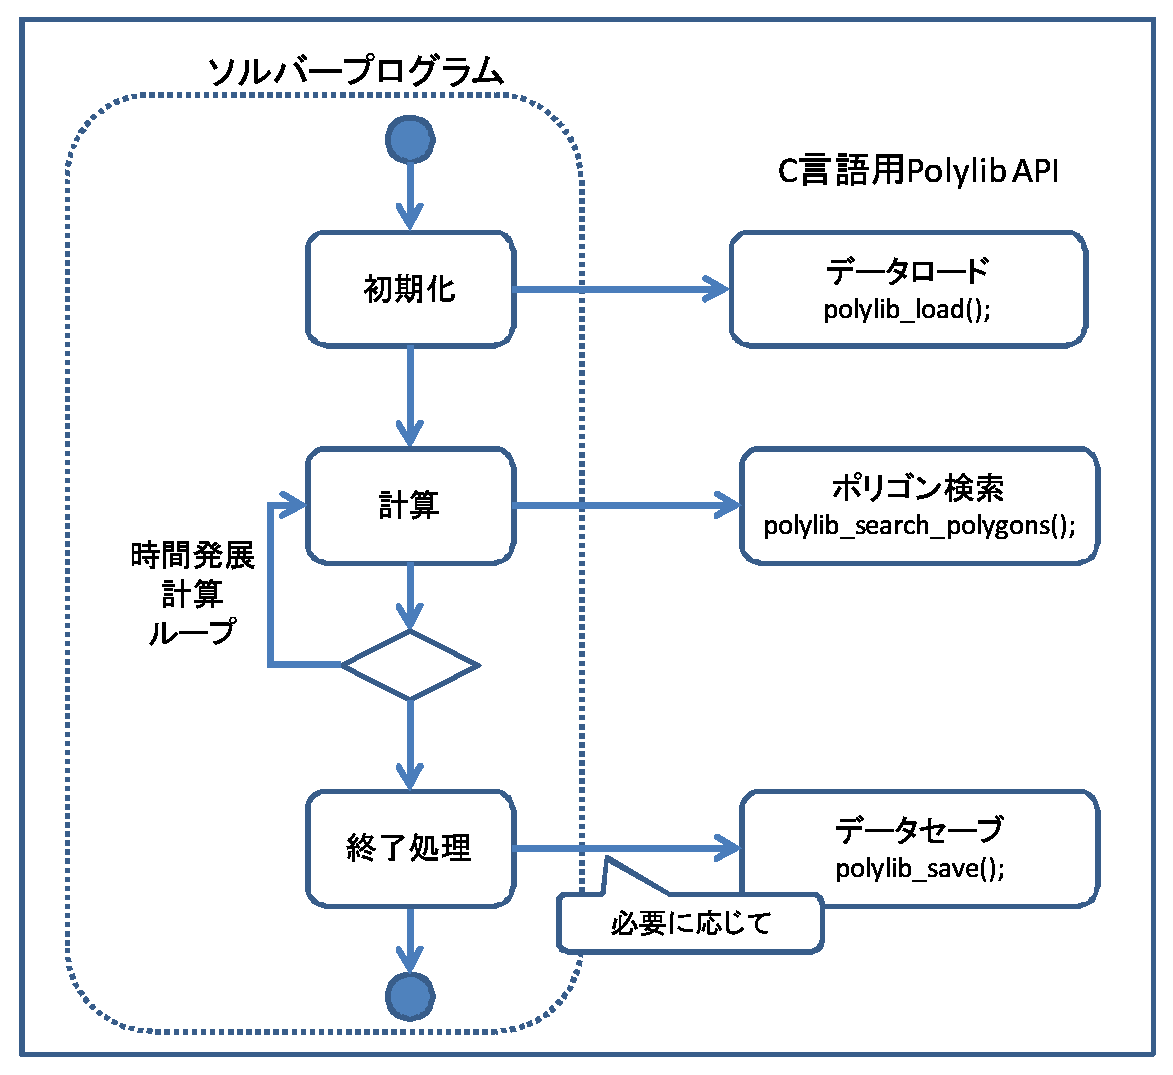
\includegraphics[width=12cm]{clip024.eps}\\
 \caption{API利用手順(C言語 単一プロセス版)}
\end{figure}

C言語用Polylibの各APIは基本的にC++版Polylibの各メソッドのラッピング関数として実現されています.
各APIの引数・返却値等はC言語向けに型変換されていること以外に違いはありません.

C言語用Polylibには,Polylib::move()相当の機能はありません.これは,Polylib::move()がクラスの
継承やメソッドの動的束縛など,オブジェクト指向プログラミングの仕組みを利用して実現されている
ためです.


\pagebreak

%
\section{C言語用Polylib 主なAPI利用方法(MPI版)}

本節ではC言語用のMPI版Polylibの主なAPI利用方法を,API呼び出し順に沿って説明します.

C言語用MPI版PolylibのAPIを利用する手順は下図の通りです.

\begin{figure}[H]
 \centering
 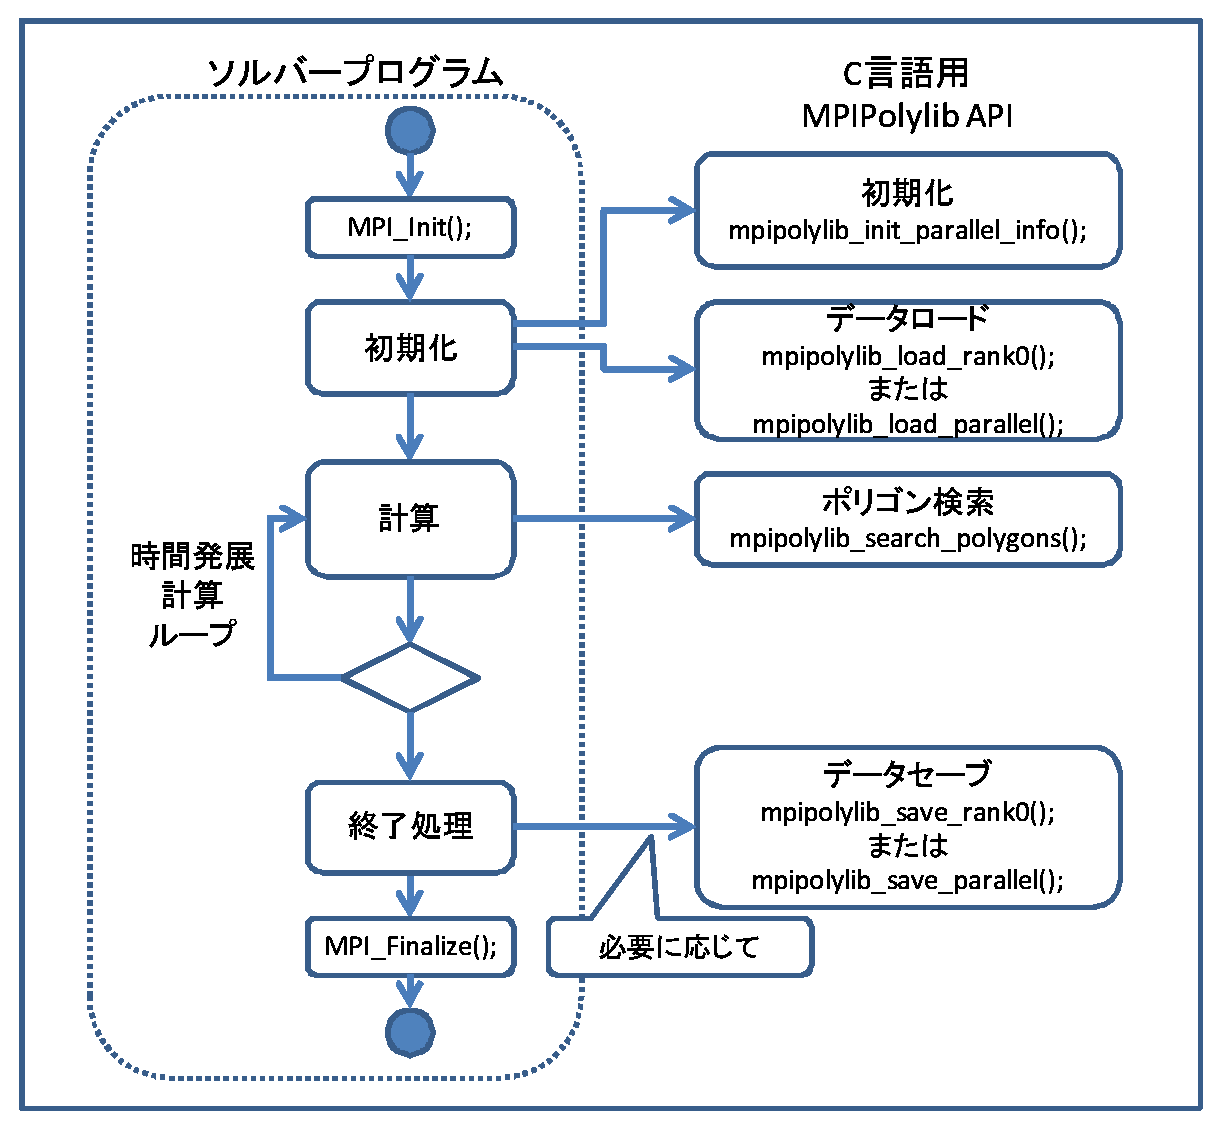
\includegraphics[width=12cm]{clip025.eps}\\
 \caption{API利用手順(C言語 MPI版)}
\end{figure}

C言語用MPIPolylibの各APIは基本的にC++版MPIPolylibの各メソッドのラッピング関数として実現されて
います.各APIの引数・返却値等はC言語向けに型変換されていること以外に違いはありません.

C言語用MPIPolylibには,MPIPolylib::move()やMPIPolylib::migrate()相当の機能はありません.これは,
これらの機能がクラスの継承やメソッドの動的束縛など,オブジェクト指向プログラミングの仕組みを
利用して実現されているためです.


\pagebreak

%
\section{動作確認用API}

本節ではPolylibおよびMPIPolylibの動作確認用APIについて説明します.これらのAPIはソルバー開発時
に利用するものであり,動作速度やメモリー消費量の点において非効率的ですので,通常のソルバー実行時
には利用しないでください.

%
\subsection{ポリゴングループ階層構造確認用API}

\begin{program}
	void Polylib::show_group_hierarchy(
		FILE	*fp = NULL
	);
\end{program}

Polylib管理下の全てのポリゴングループについて,その名称を階層レベルに従ったインデントをつけて
引数fpで指定されたファイルへ出力します.fpが未指定の場合は標準出力に出力します.

%
\subsection{ポリゴングループ情報確認用API}

\begin{program}
	void Polylib::show_group_info(std::string group_name);
\end{program}

指定された名称のポリゴングループについて,グループの情報と配下の三角形ポリゴン情報を標準出力に
出力します.

出力内容は以下の通り.

\begin{itemize}
 \item 親グループ名称
 \item 自身の名称
 \item STLファイル名
 \item 登録三角形数
 \item 各三角形の3頂点ベクトルの座標
 \item 法線ベクトルの座標
 \item 面積
\end{itemize}

%
\subsection{ポリゴン座標移動距離確認用API}

\begin{program}
	POLYLIB_STAT PolygonGroup::init_check_leaped();

	POLYLIB_STAT PolygonGroup::check_leaped(
		Vec3f	origin,
		Vec3f	cell_size
	);
\end{program}

PolygonGroup継承クラスでオーバーライドしたmove()メソッドにおいて,三角形ポリゴンの頂点座標
が隣接ボクセルより遠方へ移動したか否かをチェックするために利用するAPIです.

PolygonGroup::init\_check\_leaped()は,チェック処理の初期化関数です.move()メソッド内で,実際
に頂点移動処理を行う前に呼び出します.移動前の頂点座標を一時的に保存しますので,当該ポリゴン
グループの三角形ポリゴン数に応じてメモリを消費します.

PolygonGroup::check\_leaped()は,移動前後の頂点座標の距離を確認する関数です.move()メソッド内で,
頂点移動処理実行後に呼び出します.隣接ボクセルより遠方に移動した頂点については,標準エラー
出力にその三角形ID,移動前後の頂点座標情報を出力します.

出力例を以下に示します.

\begin{program}
PolygonGroup::check_leaped() Leaped Vertex Detected. GroupID:0 TriaID:2355
 before:(-16.0798 1093.99 -605.148) after:(-16.0798 1147.59 -496.047)
\end{program}

並列環境下で本APIを利用する場合,各ランクにおけるcheck\_leaped()の引数origin, cell\_sizeは,
MPIPolylib::get\_myproc()で取得できるParallelInfo構造体のメンバ変数m\_areaから取得することが
可能です.

なお,PolygonGroup::init\_check\_leaped()で確保された一時的メモリ領域は,PolygonGroup::check\_leaped()
を呼び出すと解放されます.

%
\subsection{メモリ消費量確認用API}

\begin{program}
	unsigned int Polylib::used_memory_size();

	unsigned int MPIPolylib::used_memory_size();
\end{program}

PolylibおよびMPIPolylibが確保しているメモリ量をbyte単位で返却します.

MPIPolylibの場合,本メソッドを呼び出したランクにおけるメモリ量が返されます.

報告されるメモリ消費量は概算です.ユーザ定義されたPolygonGroup派生クラスの拡張属性等のPolylib
フレームワーク外の消費メモリ利用については含まれません.

\pagebreak

%
\section{エラーコード}

Polylib内部でエラーが発生した場合に返却されるエラーコードPOLYLIB\_STAT型は,
include/common/PolylibStat.hに定義されています.
エラーコードの一覧を下表に示します.

\begin{table}[htbp]
\begin{tabular}{|l|l|} \hline
エラーコード & 意味 \\\hline
\hline
 PLSTAT\_OK & 処理成功 \\\hline
 PLSTAT\_NG & 一般的なエラー \\\hline
 PLSTAT\_INSTANCE\_EXISTED & Polylibインスタンスがすでに存在している \\\hline
 PLSTAT\_INSTANCE\_NOT\_EXIST & Polylibインスタンスが存在しない \\\hline
 PLSTAT\_STL\_IO\_ERROR & STLファイルIOエラー \\\hline
 PLSTAT\_UNKNOWN\_STL\_FORMAT & ファイル拡張子が.stla,.stlb,.stl以外 \\\hline
 PLSTAT\_FILE\_NOT\_SET & リーフグループにファイル名が未設定 \\\hline
 PLSTAT\_CONFIG\_ERROR & 定義ファイルでエラー発生 \\\hline
 PLSTAT\_GROUP\_NOT\_FOUND & グループ名がPolylibに未登録 \\\hline
 PLSTAT\_GROUP\_NAME\_EMPTY & グループ名が空である \\\hline
 PLSTAT\_GROUP\_NAME\_DUP & グループ名が重複している \\\hline
 PLSTAT\_MEMORY\_NOT\_ALLOC & メモリ確保に失敗した \\\hline
 PLSTAT\_POLYGON\_NOT\_EXIST & PolygonGroupにPolygonsが未設定 \\\hline
 PLSTAT\_TRIANGLE\_NOT\_EXIST & Polygonsに三角形リストが未設定 \\\hline
 PLSTAT\_NODE\_NOT\_FIND & KD木生成時に検索点が見つからなかった \\\hline
 PLSTAT\_ROOT\_NODE\_NOT\_EXIST & KD木のルートノードが存在しない \\\hline
 PLSTAT\_ARGUMENT\_NULL & 引数のメモリ確保が行われていない \\\hline
 PLSTAT\_MPI\_ERROR & MPI関数がエラーを戻した \\\hline
\end{tabular}
\caption{エラーコード一覧}
\label{tbl:error code}
\end{table}